\section{經典問題}
    \subsection{前言}
    接下來,我們會看到許多DP的經典問題。

    \subsection{費氏數列變化}
    以下問題都與費氏數列有關,但轉移式有所改變。

    \example AtCoder DP Contest A.Frog

    \textbf{題目敘述}

    有 $N$ 個石頭,編號為 $1,2,\cdots,N$。對於每個 $i \ (1 \le i \le N)$,第 $i$ 個石頭的高度是 $h_i$。

    有一隻青蛙最初位於石頭 $1$。它將重複以下動作數次,直到到達石頭 $N$:

    如果青蛙目前在石頭 $i$,則跳到石頭 $i+1$ 或石頭 $i+2$。在這裡,會產生一個代價 $|h_i - h_j|$,其中 $j$ 是要跳到的石頭。
    找到青蛙到達石頭 $N$ 之前可能產生的最小總代價。

    \textbf{輸入說明}

    輸入以以下格式從標準輸入中給出:

    $N$

    $h_1 \ h_2 \ \cdots \ h_N$

    所有輸入值均為整數。$2 \le N \le 10^5$,
    $1 \le h_i \le 10^4$

    \textbf{輸出說明}

    輸出產生的最小可能總代價。

    \textbf{範例測試}

    \begin{tabular}{|m{7cm}|m{7cm}|}
        \hline
        範例輸入 1 & 範例輸出 1 \\
        \hline
        \verb|4| & \verb|30| \\
        \verb|10 30 40 20| & \\
        \hline
        範例輸入 2 & 範例輸出 2 \\
        \hline
        \verb|6| & \verb|40| \\
        \verb|30 10 60 10 60 50| & \\
        \hline
    \end{tabular}

    \textbf{想法}

    對於這個問題我們可以遵循我們的常規方法,所以首先,我們要定義狀態。

    你認為什麼樣的狀態可以滿足我們的需求呢?如果是簡單的問題,我們可以用
    題目最後的要求定義狀態,以此題為例。題目要求找到青蛙到達石頭 $N$ 
    之前可能產生的最小總代價,因此,我們可以這樣定義。
    
    $$dp_n :=到達n產生的最小總代價$$

    接著,我們需要轉移式,題目上有提供,我們只能向前走1或2步,
    所以我們一定是從第$n-1$格或第$n-2$格走過來的。於是,從這兩種情況中找出
    最好的,便可以列出下式。

    $$
    \begin{cases}
        dp_1=0, \; dp_2=|a_1-a_2| \\
        dp_n=\min (dp_{n-1}+|a_n-a_{n-1}|,dp_{n-2}+|a_{n}-a_{n-2}|)
    \end{cases}
    $$

    其中初始狀態很是關鍵,因為第二格只能從第一格走過來,所以走到第二格只有一種方法。

    時間複雜度為$O(n)$。

    \example ZJ b587 Tri Tiling

    \textbf{題目敘述}

    給你一個 $3 \times n$ 的地面,用 $1 \times 2$ 的地板磚鋪滿,問有幾種方法。

    \textbf{輸入說明}

    每行有一個整數 $n$,代表 $3 \times n$ 的地面,$0 \leq n \leq 30$,$n=-1$ 時代表輸入結束。

    \textbf{輸出說明}

    請對每一個輸入,輸出可能的排法數。

    \textbf{範例測試}

    \begin{tabular}{|m{7cm}|m{7cm}|}
        \hline
        範例輸入 1 & 範例輸出 1 \\
        \hline
        \verb|8| & \verb|153| \\
        \verb|-1| & \\
        \hline
    \end{tabular}

    \textbf{想法}

    題目看起來很是棘手,如果遇到這種問題的時候可以考慮把紙筆拿出來。
    不過首先,同樣的,我們要定義狀態。雖然這題沒有那麼簡單,但是我們
    可以從題目的要求定義狀態開始嘗試。

    $$dp_n := 3 \times n \; 的地面,用 \; 1 \times 2 \; 的地板磚鋪滿的方法數$$

    這時候我們可能會先決定初始狀態,例如,如果$n \le 1$,則$dp_n=0$。
    如果$n=2, dp_n=3$,你可以畫圖說明這點。接著,我們發現,只要$n$是奇數,
    就不可能有任何的方法完成鋪磁磚的工作。所以我們考慮$n$是偶數的情況就可以
    了。

    \begin{figure}[!htbp]
        \centering
        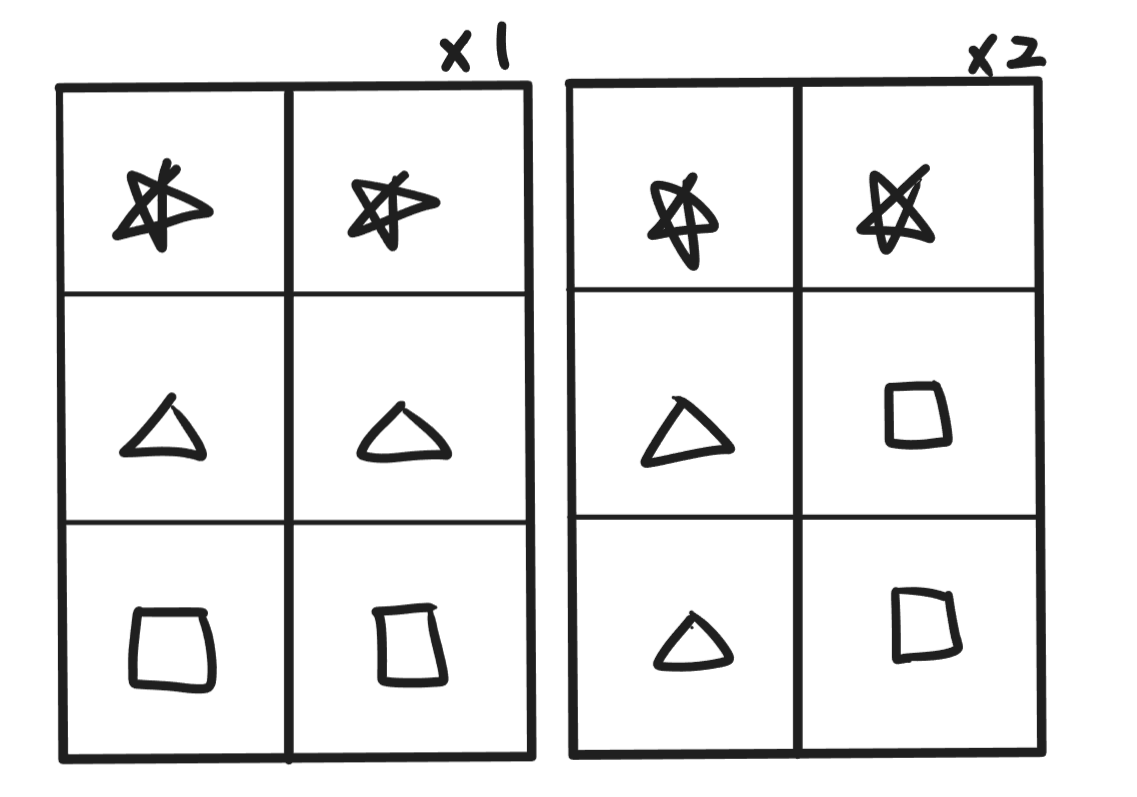
\includegraphics[width=0.5\textwidth]{../Images/DP1.png}
    \end{figure}

    \begin{figure}[!htbp]
        \centering
        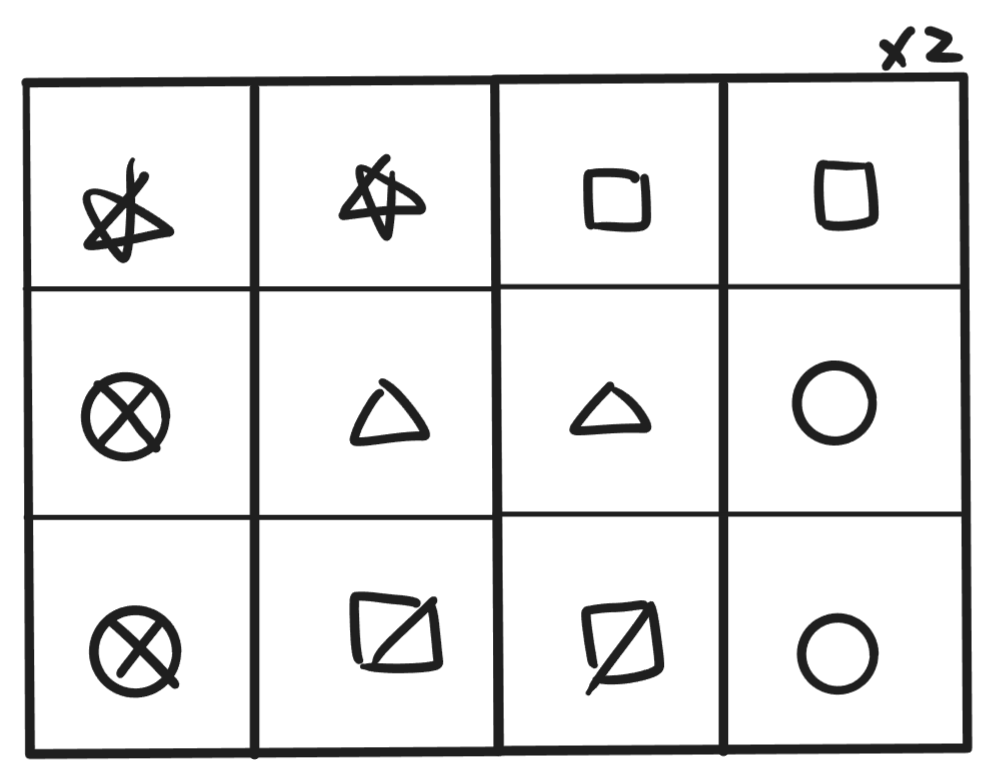
\includegraphics[width=0.5\textwidth]{../Images/DP2.png}
    \end{figure}

    根據上圖以及下頁的第一張圖片,你以為DP式像這樣。
    
    $$
    \begin{cases}
        dp_0=1, dp_2=3 \\
        dp_n=3 \times dp_{n-2}+2 \times dp_{n-4}
    \end{cases}
    $$
    
    但是當你滿心歡喜地把答案丟上去,你發現,你竟然錯了。難道還有沒有考慮到的狀態。

    這時候我們需要重新檢視自己有沒有錯誤,例如多數或少數。以這題為例我們就少數了。
    (剛剛發現的,解法也是剛剛才想,所以剛好可以成為範例)。

    \begin{figure}[!htbp]
        \centering
        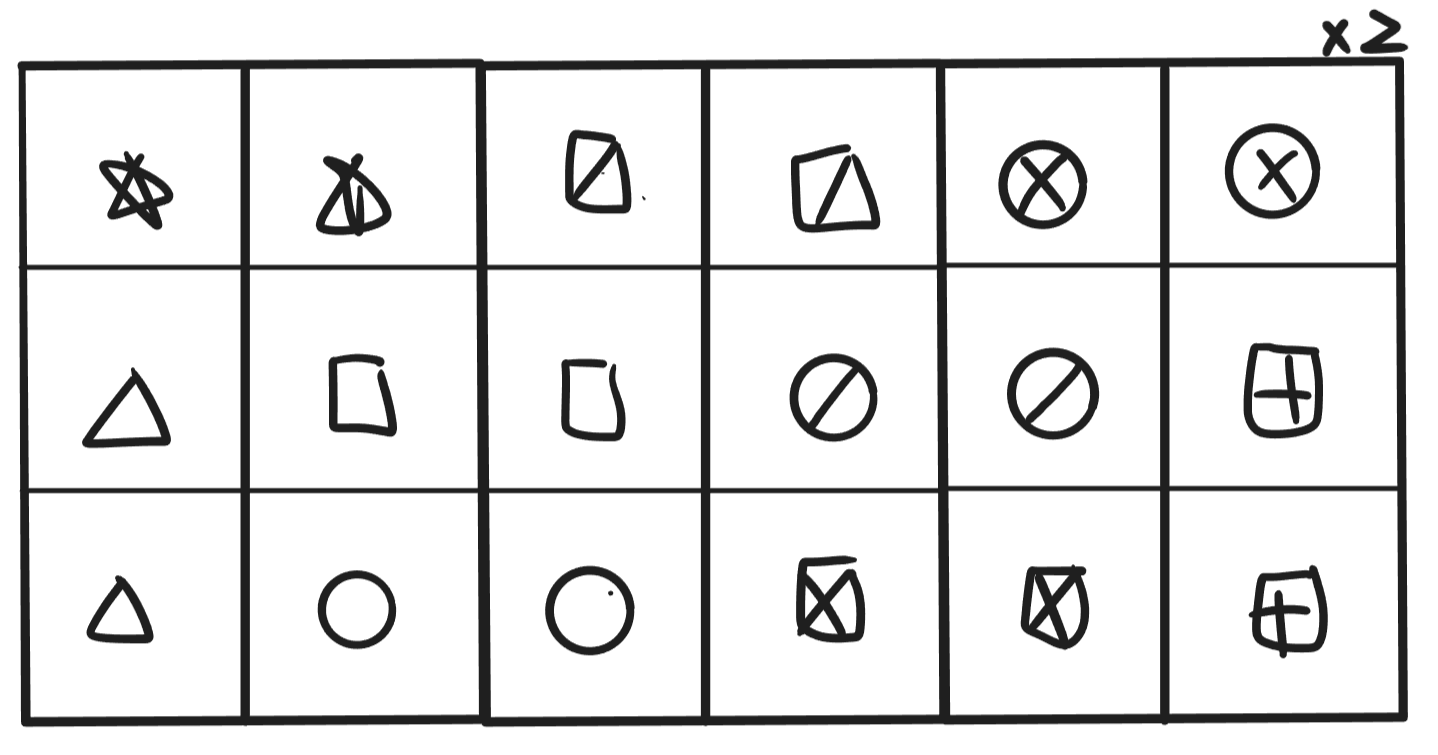
\includegraphics[width=0.8\textwidth]{../Images/DP3.png}
    \end{figure}

    依此類推,我們可得到一個新的DP式。

    $$
    \begin{cases}
        dp_0=1,dp_2=3 \\
        dp_n=3 \times dp_{n-2}+2 \times \sum_{i=1}^{\frac{n}{2}}{dp_{n-2i}}
    \end{cases}
    $$

    另外就是,雖然這題不需要,但是可以使用前綴和以及矩陣快速冪處理這個問題,
    複雜度最低為$O(\log n)$。

\begin{lstlisting}[caption=ZJ b587 題解]
#include<bits/stdc++.h>
using namespace std;

using ll=long long;

ll dp[50];

int main(){
    ios::sync_with_stdio(0);cin.tie(0);
    
    int n;

    dp[0]=1;
    dp[2]=3;
    for(int i=4;i<=30;i+=2){
        dp[i]=3*dp[i-2];
        for(int j=4;j<=i;j+=2){
            dp[i]+=2*dp[i-j];
        }
    }

    while(cin>>n && n!=-1){
        if(n&1){
            cout<<0<<"\n";
        }else{
            cout<<dp[n]<<"\n";
        }
    }
}
\end{lstlisting}

    \subsection{最長共同子序列}

    又稱為LCS(Longest Common Sequence),問題是這樣的。

    給你兩個字串,請問他們的最長共同子序列的長度,也就是
    不改變順序的話,藉由刪除某些字元讓兩格字串可以相等的
    最長長度。例如:aabbaa與aba的LCS為3。

    對於這個問題,一個變數明顯是不夠用的,所以我們可以使用
    兩個變數。首先是定義狀態,我們藉由通靈得知,可以這樣定義狀態。

    $$dp_{n,m} := 字串 \; a \; 的前 \; n \; 的字母與
    字串 \; b \; 的前 \; m \; 的字母的LCS$$

    如果這樣考慮的話,我們就可以推出轉移式。首先,如果n,m其中一個為
    0,那不可能有LCS,所以LCS一定為0。接著,對於$dp_{n,m}$,可以分為兩種情況
    字串 a 的第n的字母與字串 b  的第m的字母有沒有相等,如果相等的話,
    我們可以選擇$dp_{n-1,m-1}$,並加上1,因為加上現在的第n,m個字母相等,
    否則,只能看看前一個,這樣的情況有兩種,一種是a取前一個,另一種是b
    取前一個。

    $$
    \begin{cases}
        dp_{i,0}=dp_{0,j}=0 \\
        dp_{n,m}=\max(dp_{n-1,m}, \; dp_{n,m-1}), \; if \; a_n \ne b_m \\
        dp_{n,m}=dp_{n-1,m-1}+1, \; else
    \end{cases}
    $$
    
    實作上可以使用二維陣列。複雜度為$O(n \times m)$

\begin{lstlisting}[caption=LCS]
int dp[N][M];

int LCS(string a,string b){
    for(int i=1;i<=a.size();++i){
        for(int j=1;j<=b.size();++j){
            if(a[i-1]!=b[i-1]){
                dp[i][j]=max(dp[i][j-1],dp[i-1][j]);
            }else{
                dp[i][j]=dp[i-1][j-1]+1;
            }
        }
    }
    return dp[a.size()][b.size()];
}
\end{lstlisting}

    \subsection{最長遞增子序列}
    另一個很經典的問題就是LIS(Longest Increasing Sequence)。
    同樣是盡量刪除很少的數,以滿足剩下的數字遞增(有沒有嚴格差不多)。

    這題沒有到非常容易,首先是定義狀態,我們可以這樣定義。

    $$dp_n := 以 \; a_n \; 為結尾的 \; LIS$$

    接著,因為我們需要遞增,所以我們需要找前面所有比自己小的數字並嘗試
    接在他後面,然而,這時候我們並沒有辦法決定哪一個是最長的,
    所以必須全部都掃過一次,如此一來複雜度會是$O(n^2)$,而轉移式可以這樣寫。

    $$
    \begin{cases}
        dp_1=1 \\
        dp_n= \max(dp_{i})+1, \; i < n \; and \; a_n \ge a_i
    \end{cases}
    $$

    如果說我們只要輸出長度的話,有一個方式可以讓我們的計算速度進步到
    $O(n \log{(n)})$。我們會需要二分搜。

    \textbf{Robinson-Schensted-Knuth 算法}

    紀錄每個數字在 LIS 當中的位置。盡量往後放,因為這樣才可以接得更長。以二分搜加速搜尋位置的過程。

\begin{lstlisting}[caption=LIS 長度]
int LIS(vector<int> &v){
    vector<int> lis;
    for(int i=0;i<v.size();++i){
        int it=lower_bound(lis.begin(),lis.end(),v[i])-lis.begin();
        if(it==lis.size()){
            lis.emplace_back(v[i]);
        }else{
            lis[it]=v[i];
        }
    }
    return lis.size();
}
\end{lstlisting}

    而如果要求字典序最小的LIS,目前我只有想到一種$O(n \log(n))$的解,
    就是使用Treap查詢最小值,未來在資料結構優化當中會再次提及。

    \subsection{背包問題}

    推薦大家去看背包問題九講,裡面有好多不同情況。
    我們只會挑幾個講解。

    最經典的背包問題又稱為01背包問題,01的意思就是每樣物品只有拿或不拿兩種選項,
    其中,物品有兩種數值,$w_i$與$v_i$,而我們要最大化$v_i$的總和,且$w_i$的總和不可以大於W。
    首先我們可能會先想到窮舉所有可能性,這樣的時間複雜度為$O(2^n)$。

    但是,考慮條件:$n \le 100, W \le 10^5$,其中W是總重限制。
    顯然$2^n$不會過,所以我們需要針對這樣的情況開發新的演算法。

    首先定義狀態,既然n與W都不是很大,我們可以這樣定義。

    $$dp[n][w] := 前 \; n \; 個物品總重不大於 \; w \; 的最高價值$$

    如此一來,我們就可以設定轉移式。與LCS有些相似,都需要分為能不能拿第$i$項的情況。

    $$
    \begin{cases}
        dp[0][j] = 0 \\
        dp[i][0] = 0 \\
        dp[i][j]=dp[i-1][j], \; if \; w[i]>j \\
        dp[i][j]=\max(dp[i-1][j],dp[i-1][j-w[i]]+v[i])
    \end{cases}
    $$

    時空複雜度都是$O(nW)$,因為輸入的數據很小,所以這是可以接受的。

\begin{lstlisting}[caption=01背包]
ll dp[105][100010],v[105],w[105];

int main(){
    // input
    for(int i=1;i<=n;i++){
        for(int j=1;j<=W;j++){
            if(w[i]>j){
                dp[i][j]=dp[i-1][j];
            }else{
                dp[i][j]=max(dp[i-1][j],dp[i-1][j-w[i]]+v[i]);
            }
        }
    }
}
\end{lstlisting}
    
    接著,另一種背包問題是無限背包問題,就是每一種物品都可以拿任意數量個。
    給定 $n$ 種物品,第 $i$ 種物品重量$w_i$,價值$v_i$,背包容量 $W$
    請問最大價值($v_i$)總和為何?
    
    $n \le 100, W \le 10^5$

    對於這個問題,我們可以用相似的轉移式,因為我們的唯一差別在於能否使用
    同一個物品多次。所以我們可以將$dp[i-1][j-w[i]]+v[i]$改為$dp[i][j-w[i]]+v[i]$,
    因為$dp[i][j-w[i]]+v[i]$是包含使用過第$i$個物品的情況下的最大值。

    $$
    \begin{cases}
        dp[i][j]=dp[i-1][j], \; if \; w[i]>j \\
        dp[i][j]=\max(dp[i-1][j],dp[i][j-w[i]]+v[i])
    \end{cases}
    $$

\begin{lstlisting}[caption=無限背包]
ll dp[105][100010],v[105],w[105];

int main(){
    // input
    
    for(int i=1;i<=n;i++){
        for(int j=1;j<=W;j++){
            if(w[i]>j){
                dp[i][j]=dp[i-1][j];
            }else{
                dp[i][j]=max(dp[i-1][j],dp[i][j-w[i]]+v[i]);
            }
        }
    }
}
\end{lstlisting}

    下一個介紹的是有限背包,第$i$個物品可以拿$c_i$個。對於這樣的問題,
    我們最簡單的做法就是將第$i$個物品分成$c_i$個只能拿一次的物品,
    這樣我們就可以用01背包問題的解解開這個問題。

    然而,這樣的時空複雜度為$O(\sum{c_i} \times W)$,考慮條件$n \le 100, c_i \le 100, W \le 10^5$。
    這樣的算法會得到TLE或MLE,所以我們必須想出更有效率的做法。

    還記得快速冪嗎?同樣的方式我們也可以用在這個問題,如此一來,我們就可以
    將所有物品個切成$O(\log(c_i))$塊。這樣我們就得到$O(\sum{\log(c_i)} \times W)$。
    的解法了(利用01背包)。

\begin{lstlisting}[caption=物品切割]
using vec=vector<int>;
using pvv=pair<vec,vec>;

pvv CutItem(vector<int> &w,vector<int> &v,vector<int> &c){
    int n=w.size();
    vector<int> rw(1,0),rv(1,0);

    cin>>n;
    for(int i=0;i<n;++i){
        int c=c[i];
        for(int am=1; am<=c; c-=am,am<<=1){
            rw.emplace_back(w[i]*am);
            rv.emplace_back(c[i]*am);
        }
        
        if(c>0){
            rw.emplace_back(w[i]*c);
            rv.emplace_back(c[i]*c);
        }
    }

    return pvv{rw,rv};
}
\end{lstlisting}

    我們接著看另外一個問題。分組背包問題,題目將物品分成i組,
    總共有n個,其他限制同上。

    這時候,我們可以重新定義狀態。

    $$dp[i][j] := 前 \; i \; 組物品總重不大於 \; j \; 的最高價值$$

    而轉移式則是對每一組的所有物品都嘗試01背包的放法,
    時間複雜度為$O(nW)$。

\begin{lstlisting}[caption=分組背包]
ll dp[105][100010],v[105],w[105];

int main(){
    // input
    // 設共有k組
    for(int i=1;i<=k;i++){
        for(int u=1;u<=a[i];u++){
            for(int j=1;j<=W;j++){
                if(w[i]>j){
                    dp[i][j]=dp[i-1][j];
                }else{
                    dp[i][j]=max(dp[i-1][j],dp[i-1][j-w[i][u]]+v[i][u]);
                }
            }
        }
    }
}
\end{lstlisting}

    最後我們來看多限制背包問題,例如:今天要拿那個物品會消耗時間$t_i$,
    而你可以拿的時間只有T,同時背包有重量上限W。

    其實這個問題並沒有很困難,如果你有學會上面的背包問題,你應該可以很快的猜到,
    我們的轉移式就是對兩個限制都做一次背包。

    $$dp[n][w][t] := 前 \; n \; 個物品總重不大於 \; w \; 且時間不超過 \; t \; 的最高價值$$

    $$
    \begin{cases}
        dp[i][j][k]=dp[i-1][j][k], \; if \; w[i]>j \; or \; t[i]>w \\
        dp[i][j][k]=\max(dp[i-1][j],dp[i-1][j-w[i]][k-t[i]]+v[i])
    \end{cases}
    $$

    其時空複雜度為$O(nWT)$。

    \subsection{DAG上DP}

    我們都知道DAG是有向無環圖,因此,有時候會遇到一些問題在DAG上,通常這時候
    都可以使用DFS搭配陣列紀錄或是拓鋪排序來解決。

    \example 110宜中校內賽Final DAG上最長路徑

    \textbf{題目敘述}

    有n個點,m條邊的DAG,每個點編號為一個字串,求這個圖上的最長路徑長度。

    \textbf{輸入說明}

    第一行輸入n,m。($n \le 100, m \le 1000$)

    接下來有m行,每行有兩個字串a,b。表示有一條有向邊從a連到b。

    \textbf{輸出說明}

    DAG上最長路徑長度。

    \textbf{想法}

    當年的數據很水,可以用DFS直接過。但是我們考慮使用拓鋪排序,然後我們發現竟然可以在
    $O(n)$裡面完成。

    \subsection{範例與練習}

    \problem Atcoder DPC B Frog 2

    \textbf{題目敘述}

    有 $N$ 個石頭,編號為 $1,2,\cdots,N$。對於每個石頭 $i$ ($1\leq i\leq N$),其高度為 $h_i$。

    有一隻青蛙最初位於石頭 $1$。它將重複以下動作多次,直到到達石頭 $N$:

    如果青蛙目前在石頭 $i$,則可以跳到以下位置之一:石頭 $i+1,i+2,\cdots,i+K$。在這裡,會產生一個代價 $|h_i - h_j|$,其中 $j$ 是跳到的石頭。
    找到在青蛙到達石頭 $N$ 之前可能產生的最小總代價。

    \textbf{輸入說明}

    所有輸入值均為整數,並以以下格式呈現:

    $N$

    $K$

    $h_1,h_2,\cdots,h_N$

    $2\leq N\leq 10^5$,$1\leq K\leq 100$,$1\leq h_i\leq 10^4$

    \textbf{輸出說明}

    輸出最小可能的總花費。

    \textbf{範例測試}

    \begin{tabular}{|m{7cm}|m{7cm}|}
        \hline
        範例輸入 1 & 範例輸出 1 \\
        \hline
        \verb|5 3| & \verb|30| \\
        \verb|10 30 40 50 20| & \\
        \hline
    \end{tabular}

    \problem Atcoder DPC C Vacation

    \textbf{題目敘述}

    Taro的暑假明天開始,他決定現在就為它做計劃。

    這個假期有 $N$ 天。對於每一天 $i$ $(1 \le i \le N)$,Taro將選擇以下其中一個活動,並在第 $i$ 天做:

    A:在海裡游泳。獲得 $a_i$ 點快樂值。
    B:在山上捉蟲子。獲得 $b_i$ 點快樂值。
    C:在家做作業。獲得 $c_i$ 點快樂值。
    由於Taro容易感到無聊,他不能連續兩天做相同的活動。

    找出Taro所獲得的最大可能總快樂值。

    \textbf{輸入說明}

    所有輸入值都是整數。

    輸入格式如下:

    $N$

    $a_1 \quad b_1 \quad c_1$

    $a_2 \quad b_2 \quad c_2$

    $\vdots$

    $a_N \quad b_N \quad c_N$

    $1 \le N \le 10^5$,$1 \le a_i, b_i, c_i \le 10^4$

    \textbf{輸出說明}

    輸出Taro所獲得的最大可能總快樂值。

    \textbf{範例測試}

    \begin{tabular}{|m{7cm}|m{7cm}|}
        \hline
        範例輸入 1 & 範例輸出 1 \\
        \hline
        \verb|3| & \verb|210| \\
        \verb|10 40 70| & \\
        \verb|20 50 80| & \\
        \verb|30 60 90| & \\
        \hline
    \end{tabular}

    \problem Atcoder DPC E Knapsack 2

    \textbf{題目敘述}

    有 $N$ 個物品,編號從 $1$ 到 $N$。對於每個 $i$ ($1 \le i \le N$),物品 $i$ 的重量為 $w_i$,價值為 $v_i$。

    Taro決定在一個背包中選擇一些物品並攜帶回家。背包的容量為 $W$,這意味著所選物品的重量總和必須不超過 $W$。

    找出 Taro 攜帶回家的物品價值的最大可能總和。

    \textbf{輸入說明}

    所有輸入值都是整數。

    輸入格式如下:

    $N\ W$

    $w_1\ v_1$

    $w_2\ v_2$

    $\vdots$

    $w_N\ v_N$

    $1 \le N \le 100$

    $1 \le W \le 10^9$

    $1 \le w_i \le W$

    $1 \le v_i \le 10^3$

    \textbf{輸出說明}

    輸出 Taro 攜帶回家的物品價值的最大可能總和。

    \textbf{範例測試}

    \begin{tabular}{|m{7cm}|m{7cm}|}
        \hline
        範例輸入 1 & 範例輸出 1 \\
        \hline
        \verb|3 8| & \verb|90| \\
        \verb|3 30| & \\
        \verb|4 50| & \\
        \verb|5 60| & \\
        \hline
    \end{tabular}

    \problem Atcoder DPC F LCS

    \textbf{題目敘述}

    給定兩個字符串
    $s$ 和
    $t$。找出一個最長的字符串,它同時是
    $s$ 和
    $t$ 的子序列。

    備註
    字符串
    $x$ 的子序列是通過從
    $x$ 中刪除零個或多個字符並連接剩下的字符而獲得的字符串,而且不改變字符的順序。

    \textbf{輸入說明}

    輸入以以下格式給出:

    $s$

    $t$

    $s$ 和 $t$ 是由小寫英文字母組成的字符串。
    $1\le |s|, |t|\le 3000$

    \textbf{輸出說明}

    輸出一個最長的字符串,它是
    $s$ 和
    $t$ 的子序列之一。如果有多個這樣的字符串,可以接受任意一個。

    \textbf{範例測試}

    \begin{tabular}{|m{7cm}|m{7cm}|}
        \hline
        範例輸入 1 & 範例輸出 1 \\
        \hline
        \verb|axyb| & \verb|axb| \\
        \verb|abyxb| & \\
        \hline
    \end{tabular}

    \problem Atcoder DPC H Grid 1

    \textbf{題目敘述}

    給定一個網格,包含 $H$ 個水平行和 $W$ 個垂直列。我們用 $(i,j)$ 表示網格中第 $i$ 行和第 $j$ 列的方格。

    對於每個 $(i,j)$,方格 $(i,j)$ 的內容用字符 $a_{i,j}$ 表示。如果 $a_{i,j}$ 是\verb|.|,表示方格 $(i,j)$ 是一個空方格;如果 $a_{i,j}$ 是\verb|#|,表示方格 $(i,j)$ 是一個牆方格。保證方格 $(1,1)$ 和 $(H,W)$ 是空方格。

    Taro 從方格 $(1,1)$ 出發,每次可以向右或向下移動到相鄰的空方格,目標是到達 $(H,W)$。

    求從方格 $(1,1)$ 到 $(H,W)$ 的 Taro 路徑數量。由於答案可能非常大,請將結果對 $10^9 + 7$ 取模。

    \textbf{輸入說明}

    輸入以以下格式給出:

    $H$
    $W$
    $a_{1,1} \cdots a_{1,W}$
    
    $\vdots$
    
    $a_{H,1} \cdots a_{H,W}$

    $H$ 和 $W$ 為整數。
    $2 \le H, W \le 1000$
    $a_{i,j}$ 為\verb|.|或\verb|#|。
    方格 $(1,1)$ 和 $(H,W)$ 是空方格。

    \textbf{輸出說明}

    輸出從方格 $(1,1)$ 到 $(H,W)$ 的 Taro 路徑數量,對 $10^9 + 7$ 取模。

    \textbf{範例測試}

    \begin{tabular}{|m{7cm}|m{7cm}|}
        \hline
        範例輸入 1 & 範例輸出 1 \\
        \hline
        \verb|3 4| & \verb|3| \\
        \verb|...#| & \\
        \verb|.#..| & \\
        \verb|....| & \\
        \hline
    \end{tabular}

    \problem ZJ b589 超級馬拉松賽

    \textbf{題目敘述}

    一個超級馬拉松比賽將開始。在遊戲中,選手每天需要跑不同的路徑。
    假設遊戲全部有 n 條路徑; 每個路徑得分可以是不同的。
    如果一名選手不能在規定時間內完成一條路徑,他該路徑得到零分;
    如果玩家完成了一條路徑在一個規定的時間,他得到該路徑設定的得分;
    如果玩家完成了一條路徑,用較短的時間,他可以得兩倍分數。

    小愛想參加這個比賽,她如果在一條路徑上按正常速度來跑,
    就只能拿到原始分數,如果他加速跑,就能拿到兩倍分數,
    不過她就會需要在加速跑完後的下一條路徑上休息而速度變慢得到0分,
    請寫一個程式幫助小愛計算哪些路徑應該加速得到兩倍分數而能獲得最高的總得分。

    \textbf{輸入說明}

    輸入資料包含多組測試資料,每一組測試資料有兩行,第一行有一個數字 n 代表有 n 條路徑要跑 $1 \le n \le 40$,第二行有 n 個整數代表每個路徑的原始得分 $10 \le P1, P2, \cdots , Pn \le 100$

    當 n 為 0 時代表輸入結束。

    \textbf{輸出說明}

    對每一組測試資料輸出最好的總得分,每一筆資料輸出一行。

    \textbf{範例測試}

    \begin{tabular}{|m{7cm}|m{7cm}|}
        \hline
        範例輸入 1 & 範例輸出 1 \\
        \hline
        \verb|3| & \verb|210| \\
        \verb|90 60 10| & \\
        \verb|0| & \\
        \hline
    \end{tabular}

    \begin{tip}
        請考慮增加狀態,或是讓狀態有附加定義。
    \end{tip}

    \problem CF 455A Boredom
    
    \textbf{題目敘述}

    Alex 不喜歡無聊。所以每當他感到無聊,他就會想出遊戲來玩。一個漫長的冬夜,他想出了一個遊戲,決定玩一下。

    給定一個由 $n$ 個整數組成的序列 $a$。玩家可以進行多個步驟。在一個步驟中,他可以選擇序列中的一個元素(假設為 $a_k$)並刪除它,同時必須刪除所有等於 $a_{k+1}$ 和 $a_{k-1}$ 的元素。這一步給玩家帶來 $a_k$ 個分數。

    Alex 是一個完美主義者,所以他決定盡可能地獲得最多的分數。請幫助他。

    \textbf{輸入說明}

    第一行包含一個整數 $n$($1 \le n \le 10^5$),表示 Alex 的序列中有多少個數字。

    第二行包含 $n$ 個整數 $a_1, a_2, \cdots, a_n$($1 \le a_i \le 10^5$)。

    \textbf{輸出說明}

    輸出一個整數,表示 Alex 可以獲得的最大分數。

    \textbf{範例測試}

    \begin{tabular}{|m{7cm}|m{7cm}|}
        \hline
        範例輸入 1 & 範例輸出 1 \\
        \hline
        \verb|9| & \verb|10| \\
        \verb|1 2 1 3 2 2 2 2 3| & \\
        \hline
    \end{tabular}

    \begin{tip}
        狀態比較特殊,觀察數字範圍。
    \end{tip}